\chapter{Mathematical Considerations}
\label{ch:math}

\section{Zipf's laws in RecSys and the Matthew Effect}

In a great many applications of machine learning, a caveat is given early, that the distribution of observations of unique items from a large corpus is modeled by Zipf's law. In recommendation systems, the \emph{Matthew Effect} appears in the popular item's click rates, or the popular user's feedback rates. 

Simply, the Matthew Effect–or popularity bias–states that the most popular items continue to attract the most attention and widen the gap with other items. Take for example the MovieLens dataset, an extremely popular dataset for benchmarking recommendation systems[link to MovieLens info], in [[Jenny Sheng 2020]\url{https://jennysheng.com/jenny-sheng-iw-fall-2020.pdf}] they observe the following behavior for number of movie ratings:

\vspace{10pt}
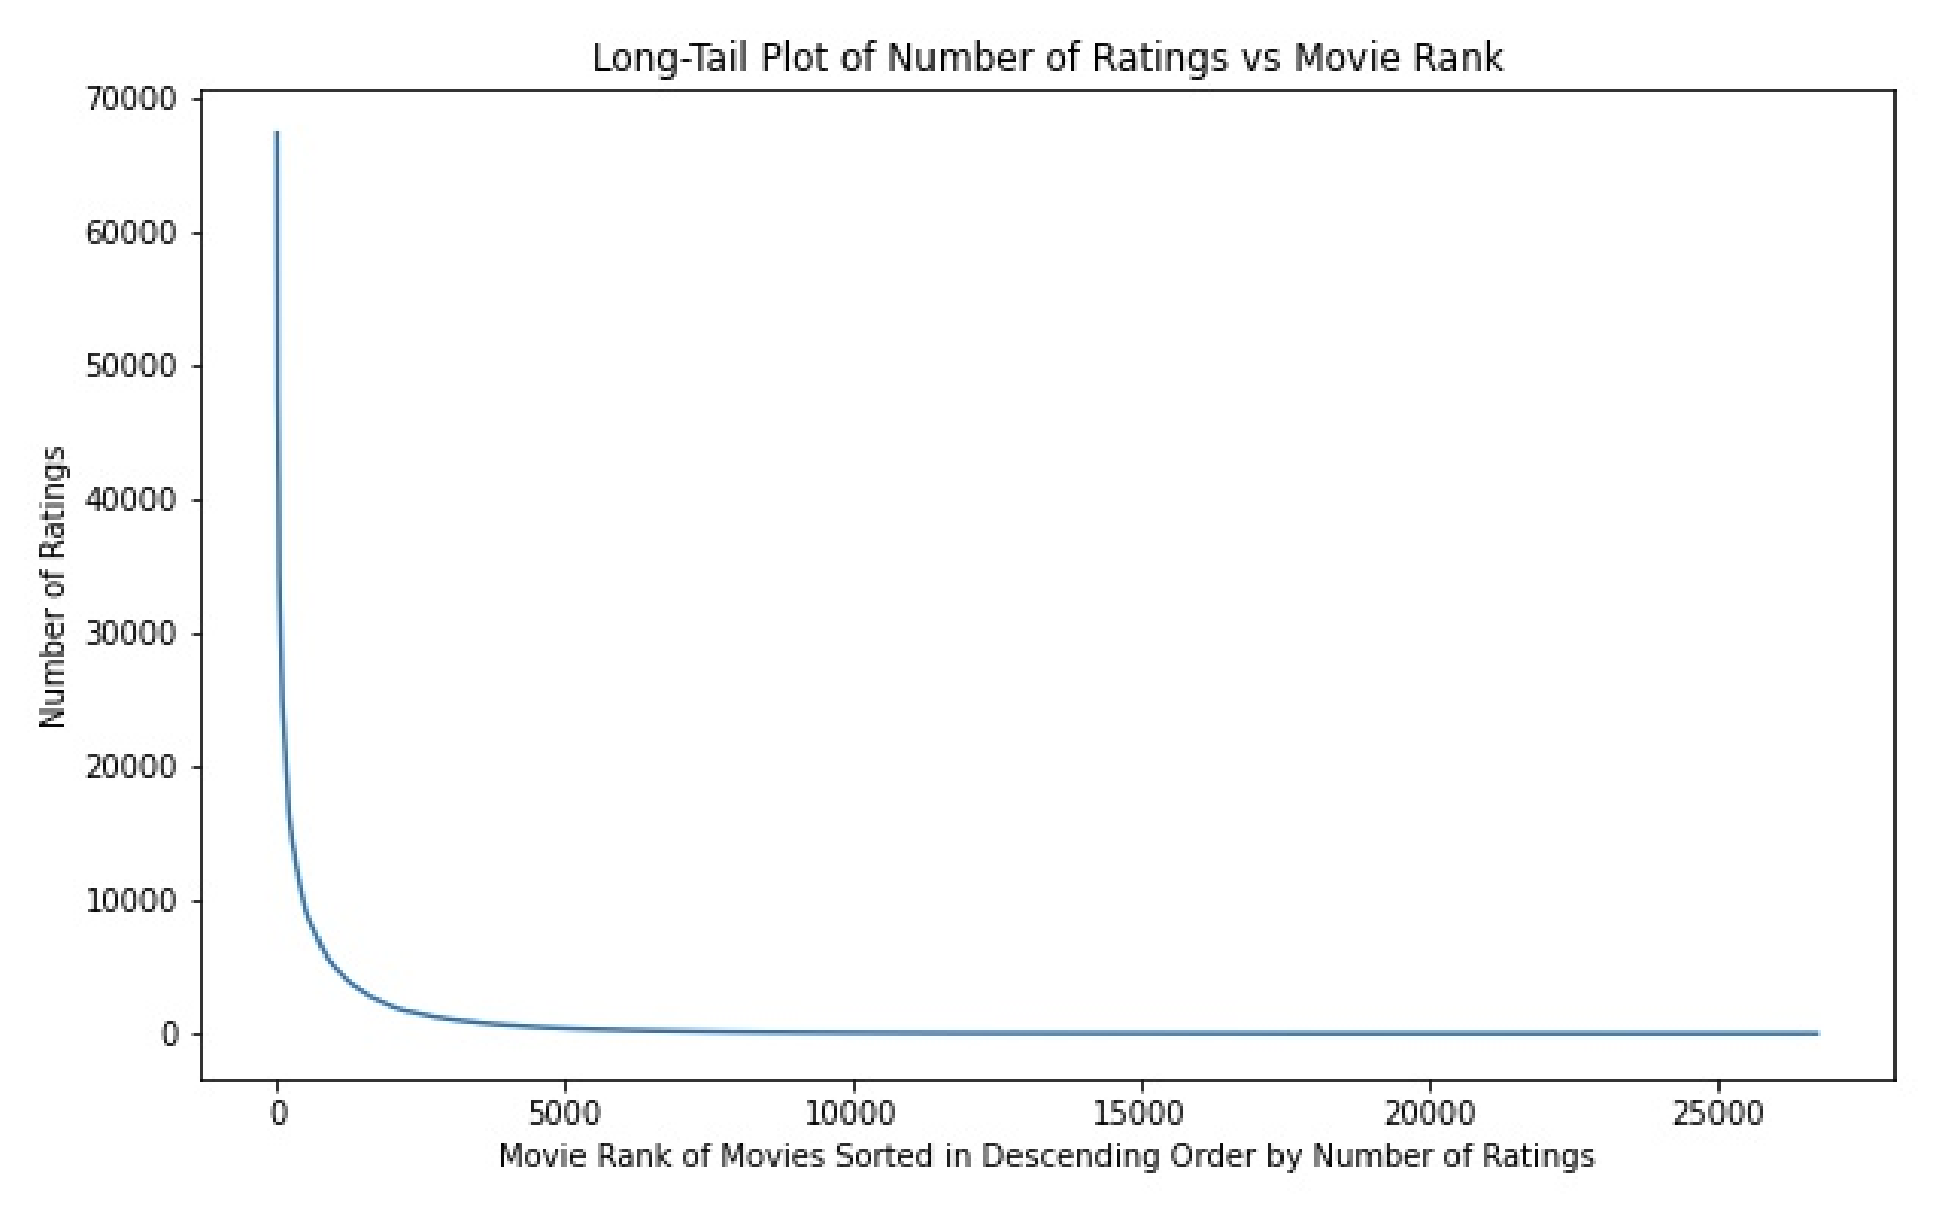
\includegraphics[width=\textwidth-10pt]{book-text/zipfian-moverank.png}

At first glance this behavior is obvious and stark, but is it a problem? Let's assume our recommender will be built as a user-based CF model–as alluded to in \ref{ch:user-item}–then how might these distributions effect the recommender?

Let the probability mass function be described by the simple Zipf's law:

\begin{equation}
    f(k, M) = \frac{1/k}{\sum^M_{n=1}(1/n)}    
\end{equation}


for $M$ number of tokens in the corpus (in the above examples number of movies), $k$ is the rank of a token when sorted by number of occurrences. 

Let's consider users $A$ and $B$, with $N_A = \mathcal{I}_A$  and $N_B = \mathcal{I}_B$ ratings respectively, Observe that the probability of $V_i$, the $i$'th most popular video, appearing in $\mathcal{I}_X$ for some user $X$ is given by:
\begin{equation}
    P(i)=\frac{f(i,M)}{\sum^M_{j=1}f(j,M)}=\frac{1/i}{\sum^M_{j=1}1/j}
\end{equation}

and thus the joint probability of an item appearing in two user's ratings is:

\begin{equation}
  P(i^2)=\left(\frac{1/i}{\sum^M_{j=1}1/j}\right)^2.  
\end{equation}

This becomes important when one also considers that our, yet unstated, definition of user-based collaborative filtering, is based on similarity in user's ratings sets–\emph{number of jointly rated items by two users, divided by the total number of items rated by either.}

Taking this definition, we can for example, compute the similarity score for one shared item amongst $A$ and $B$:

\begin{equation}
    \sum^M_{i=1} \frac{P(i^2)}{\| \mathcal{I}_A \cup \mathcal{I}_B \|},
\end{equation}

and the average similarity score of two users is generalized to:

\begin{equation}
    \sum^{\min(N_A,N_B)}_{t=1}\left(\prod_{i_k=i_{k-1}+1}^{t-1}\sum^M_{i=1} \frac{P({i_k}^2)}{\frac{\| \mathcal{I}_A \cup \mathcal{I}_B \|}{t}}\right).
\end{equation}

These combinatorial formulas indicate not only the relevance of the Zipfian in our algorithms, but we see an almost direct effect on the output of scores. Consider the experiment from [(Wang, Wang, and Zhang 2019)]\url{https://arxiv.org/abs/1909.12798}; for LastFM users, the authors demonstrate average similarity scores for pairs of users, and they find this Matthew Effect persists into the similarity matrix:

\vspace{10pt}
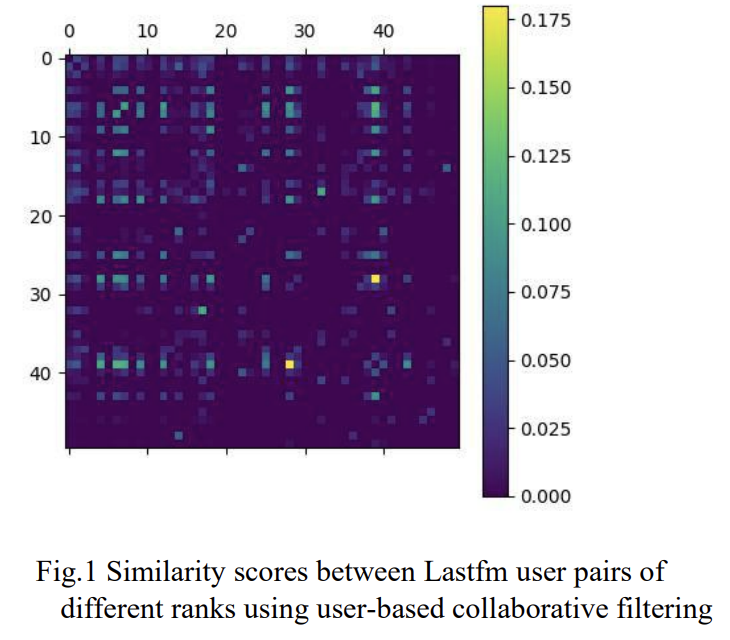
\includegraphics[width=\textwidth-10pt]{book-text/lastfm-matthew-effect.png}

While these results might seem scary, we'll observe later via diversity-aware loss functions that we can mitigate some of this. An even simpler way, is to use downstream sampling methods, which we will discuss as part of our explore-exploit algorithms. Finally, the Matthew Effect is only the first of two major impacts of this Zipfian–let's turn our attention to the second.


\section{Sparsity}

We now must reckon with sparsity. As the ratings skew more and more towards the most popular items, the least popular items a starved for data and recommendations, which is called \emph{Data Sparsity.} This connects to the linear algebraic definition of sparsity, mostly zeros or not populated elements in a vector, when you consider again our user-item matrix less popular items constitute columns with very few entries–these are sparse vectors. Similarly, at scale we see that the Matthew effect pushes more and more of the total ratings into certain columns, and the matrix becomes sparse in the traditional mathematical sense. For this reason, sparsity is an extremely well known challenge for recommendation systems. 

Like above, let's consider the implication on our collaborative filtering algorithms from these sparse ratings. Again observe that the probability of $V_i$, the $i$'th most popular item, appearing in $\mathcal{I}_X$ for some user $X$ is given by:

\begin{equation}
    P(i)=\frac{f(i,M)}{\sum^M_{j=1}f(j,M)}=\frac{1/i}{\sum^M_{j=1}1/j}
\end{equation}

then 

$$(M-1)*P(i)$$

is the expected number of other users which click the $i$'th most popular item, so summing over all $i$ yields the total number of other users that will share a rating with $X$:

\begin{equation}
    \sum_{i=1}^M (M-1)*P(i)
\end{equation}

Again, as we pull back to the overall trends, we observe this sparsity sneaking into the actual computations for our collaborative filtering algorithms, consider the trend of users of different ranks, and how much their rankings are used to 'collaborate' in other user's rankings:

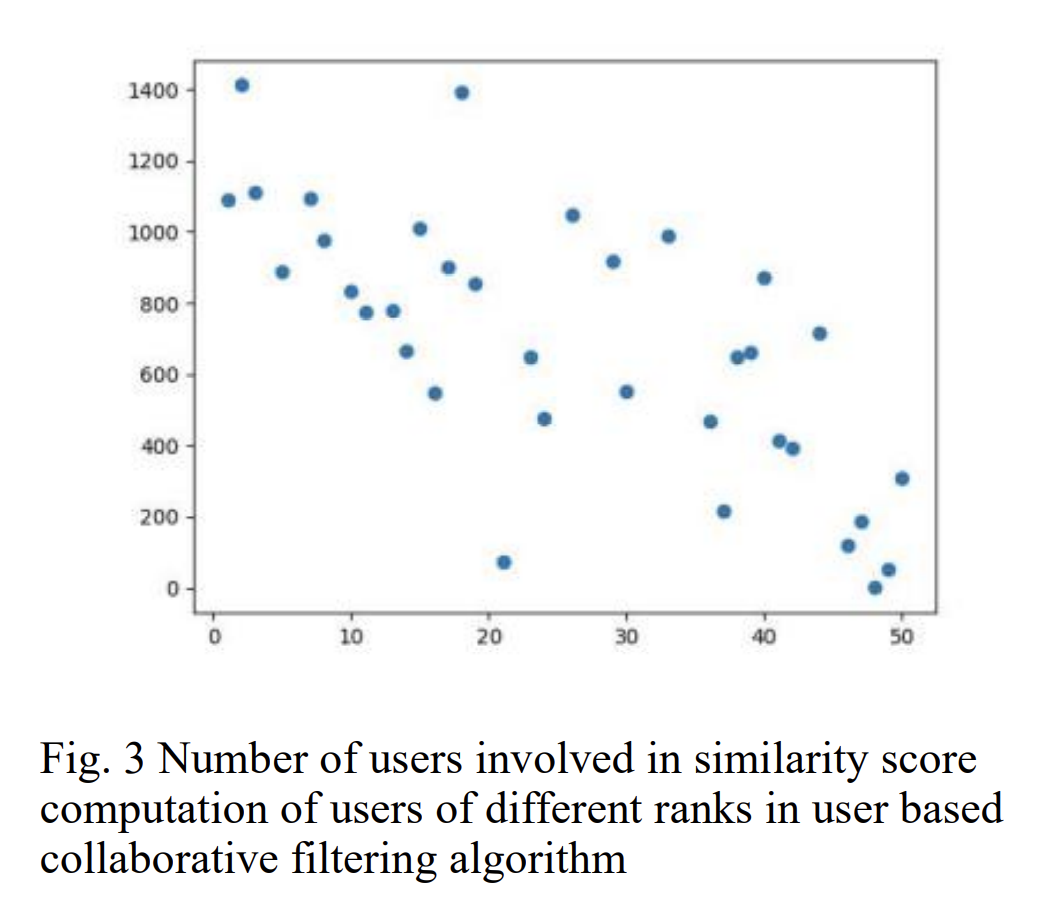
\includegraphics[width=\textwidth-10pt]{book-text/user-sim-counts.png}

We see that this is an important result to always beware–sparsity pushes emphasis onto the most popular users, and has the risk of making your recommender myopic. 

\subsection{Item-based collaborative filtering}

While the equations are different, everything above applies similarly to item-based collaborative filtering. We see similarity in items exhibit the same inheritance of the Zipfian in their scores, and we see items consulted in the collaborative filtering process drops off by rank. 

\section{User Similarity for Collaborative filtering}

In mathematics, it's most common to hear discussion of \emph{distances}–even back to the Pythagorean theorem, we are taught to think of relationships between points as distances, or dissimilarity. Indeed, this fundamental idea is canonized in mathematics as part of the definition of a metric:
\begin{itemize}
    \item $d(a,c)\leq d(a,b)+d(b,c)$
\end{itemize}


In machine learning; we often instead concern ourselves with the notion of similarity–an extremely related topic. In many cases, one can directly pass back and forth between similarity and dissimilarity; when $d:X\times X\rightarrow [0,1]\subset\mathbb{R}$ then we often define:

\begin{equation}
    Sim(a,b):=1-d(a,b)
\end{equation}

This may seem like a needlessly precise statement, but in fact we'll see that there are a [variety of options for how to frame similarity]\url{https://en.m.wikipedia.org/wiki/Similarity_measure}. Furthermore, sometimes we even formulate similarity measures where the associated distance measure does not establish a metric on the set of objects. These so-called pseudo-spaces can still be incredibly important, and we'll see where they come up in the later section on latent spaces. 

In the literature, you'll find a very common practice of papers starting by introducing a new similarity measure, and then training a model you've seen before on the new similarity measure. As we'll see, choices in how you choose to relate objects(users, items, features, etc.) can have a large effect on what your algorithms learn. 

For now, let's laser in on some specific similarity measures. Consider a classic ML problem of clustering; we have a space (usually $\mathbb{R}^n$) in which our data is represented and we are asked to partition our data into sub-collections of the population and assign these collections names. Frequently, these collections are intended to capture some meaning, or at the very least be useful for summarizing the collection elements' features. When you do that clustering, you frequently are considering points near to one another in that space. Further, if you're given a new observation, and asked to assign it to a collection as an inference task you normally compute the new observation's \emph{nearest neighbors}. This could be the k-nearest neighbors, or simply the nearest neighbor amongst cluster centers; either way, your task is to use the notion of similarity to associate. In collaborative filtering, this same notion is used to relate a user for whom you wish to make recommendations, to those you already have data from. 

So how may we define similarity for our users in collaborative filtering? They're not obviously in the same space, so our usual tools seem to be lacking. 

\subsection{Pearson correlation}

Our original formulation of Collaborative Filtering was to say that users with similar taste collaborate to recommend items for each other. Let two users $A$ and $B$, have a set of co-rated items–simply the set of items with ratings from each–written $\mathcal{R}_{A,B}$, and a rating of item $x$ by user $A$ written as $r_{A,x}$, then 

\begin{equation}
    \sum_{x\in \mathcal{R}_{A,B}}(r_{A,x}-\bar{r}_A)
\end{equation}

is the average deviation from $A$'s average rating over all of its co-rated items with $B$. If we think of these ratings as a random variable, and consider the analog for $B$, then the correlation between the jointly distributed variables, i.e. the population covariance, is our \emph{Pearson correlation:}

\begin{equation}
USim_{A,B}=\frac{\sum_{x\in \mathcal{R}_{A,B}}(r_{A,x}-\bar{r}_A)(r_{B,x}-\bar{r}_B)}{\sqrt{\sum_{x\in \mathcal{R}_{A,B}}(r_{A,x}-\bar{r}_A)^2} \sqrt{\sum_{x\in \mathcal{R}_{A,B}}(r_{B,x}-\bar{r}_B)^2}}    
\end{equation}

It's extremely important to keep in mind a few details here:

- This is the similarity of the jointly distributed variables describing the users' ratings
- We compute this via all co-rated items, so user similarity, is defined via item-ratings
- This is a pairwise similarity measure taking values in $[-1,1]\in \mathbb{R}$

\subsection{Ratings via similarity}

Now that we've introduced user-similarity, let's use it!

For a user $A$, and item $x$, we can estimate the rating via similar users' ratings:

\begin{equation}
    Aff_{A,i}=\bar{r}_A+\frac{\sum_{U\in \mathcal{N}(A)}USim_{A,U}*(r_{U,i}-\bar{r}_A)}{\sum_{U\in \mathcal{N}(A)}USim_{A,U}}
\end{equation}

This is the prediction for user $A$'s rating of item $x$, which takes $A$'s average adjusted rating of the similarity-weighted average ratings of all of $A$'s neighbors. In other words: $A$'s rating will probably be the average of people like $A$'s rating, adjusted to how generous $A$ is with ratings in general.

But wait! What's $\mathcal{N}(A)$? It's the neighborhood of $A$, via our $USim$ definition above. How many neighbors? How do you pick those neighbors? These will be the subject of later chapters; for now, assume they're $k$-nearest neighbors and assume some hyperparameter tuning is used to determine a good value for $k$.

\subsection{Fun aside:}

You might wonder, "does this Pearson correlation yield a metric space under some transformation?". The answer is yes, but it's a bit more complicated than our simple definition above. While the above can get us a distance, it's not good enough to get us a metric space, without a more novel transformation.

In particular, for $P(A,B)$ the above defined correlation, then $1-P(A,B)$ yields a distance that satisfies all metric properties *except* the triangle inequality. There are several known ways to adjust this though: $\sqrt{1-P(A,B)^2}$ being the most common. For a survey, see ([Dongen and Enright, 2012]\url{https://arxiv.org/pdf/1208.3145.pdf})

\section{Explore–exploit as a RecSys}

In the previous we saw two ideas, slightly in contrast to one another:

\begin{itemize}
\item The MPIR, a simple easy to understand recommender
\item The Matthew effect in recommendation systems, and it's runaway behavior in distributions of ratings
\end{itemize}

By now, it's likely that you realize that the MPIR will amplify the Matthew effect, and that the Matthew effect will drive the MPIR to the Trivial recommender in the limit. This is the classic difficulty of maximizing a loss function with no randomization–it very quickly settles into a mode.

This problem–and many others like it–encourage some modification to the algorithm to prevent this failure mode, and continue to expose the algorithm and users to other options. The basic strategy for \emph{explore-exploit schemes,} or \emph{multi-armed bandits} as they're called, is to take not only the outcome-maximizing recommendation, but also a collection of alternative \emph{variants,} and randomly determine which to use as response. 

Taking a step back: given a collection of variant recommendations, or \emph{arms}, $A$, for which the outcome of each recommendation is $y_t$, and we have a prior reward function $R(y_t)$. The bandit–called an \emph{agent} in this literature–would like to maximize $R(y_t)$, but the agent doesn't know the distribution of the outcomes $Y_{a\in A}$. The agent thus assumes some prior distributions for $Y_{a\in A}$, and then collects data to update those distributions; after sufficient observations, the agent can estimate the expected values of each distribution, $\mu_{a\in A}=\mathbb{E}(\mathcal{R}(Y_a))$. If the agent was able to confidently estimate these reward values, the recommendation problem would be solved: at inference, the agent would simply estimate the reward values for all variants for the user, and select the reward-optimizing \emph{arm.} This is of course ridiculous in totality, but the basic idea is useful nonetheless: hold prior assumptions about what will be greatest expected reward, and explore alternatives with some frequency to continue to update the distributions and refine your estimators.

\subsection{$\epsilon$-greedy}

So how often should you explore vs. use your reward-optimizing arm? The first best algorithm is $\epsilon$-greedy; for $\epsilon \in (0,1)$, at each request the Agent has probability $\epsilon$ of choosing a random arm and probability $1-\epsilon$ of selecting the currently highest estimated reward arm.

Let's take the MPIR and slightly modify it to include some exploration. 

\begin{lstlisting}[language=Python]
import random

def get_item_popularities() -> Optional[Dict[str, int]]:
	...
		return item_choice_counts # Dict of pairs: (item-identifier, count item chosen)
  return None

def get_most_popular_recs_ep_greedy(
	max_num_recs: int, 
	epsilon: float
) -> Optional[List[str]]:
	assert epsilon<1.0
	assert epsilon>0

	items_popularity_dict = get_item_popularities() # type: Optional[Dict[str, int]]
	if items_popularity_dict:
		sorted_items = sorted(
			items_popularity_dict.items(), 
			key=lambda item: item[1]),
			reverse=True,
		)
		top_items = [i[0] for i in sorted_items]
		recommendations = []
		for i in range(max_num_recs): # we wish to return max_num_recs
			if random.random()>epsilon: # if greater than epsilon, exploit
				recommendations.append(top_items.pop(0))
			else: # otherwise, explore
				explore_choice = random.randint(1,len(top_items))
				recommendations.append(top_items.pop(explore_choice))
		return recommendations
  return None
\end{lstlisting}

The only modification to our MPIR is that now we have two cases for each potential recommendation from our \lstinline{max_num_recs}; if a random probability is less than our $\epsilon$ then we proceed as before and select the most-popular, otherwise we select a random recommendation. 

Note that we're interpreting maximization of reward as selecting most-popular items. This is an important assumption, and as we move into more complicated recommenders, this will be the crucial assumption that we modify to get different algorithms and schemes.

\paragraph{Collector}

The collector here need not change, we still want to get the item popularities first.

\paragraph{Ranker}

The ranker also does not change! We begin by ranking the possible recommendations by popularity.

\paragraph{Server}

If collector and ranker remain the same, then clearly the server is what must be adapted for this new recommender. This is the case, instead of taking the top items to fill \lstinline{max_num_recs} we now utilize our $\epsilon$ to determine at each step if the next recommendation added to our list should be next in line from the ranker, or a random selection. Otherwise, we adhere to the same API schema, and return the same shape of data.

\subsection{What should $\epsilon$ be?}

In the above, $\epsilon$ is a fixed number for the entire call, but what should the value be? This is actually an area of great study and the general wisdom is to start with large $\epsilon$ (to encourage more exploration) and then reduce over time. The rate at which you decrease it, the starting value, and so on, require serious thought and research. Additionally, it can be tied into your prediction loop and be part of the training process.

\section{The NLP-RecSys relationship}

Let's utilize some intuition from a different area of Machine Learning, Natural Language Processing. One of the fundamental models in NLP is word2vec; a sequence–based model for language understanding that utilizes the words which co-occur in sentences together. 

For skipgram-word2vec, the model takes sentences of words, and attempts to learn the implicit meaning of words via their co-occurrence relationships with other words in those sentences. Each pair of co-occurring words, constitutes a sample that is 1-hot encoded and sent into a vocabulary-sized layer of neurons, with a bottleneck layer, and a vocabulary-sized output layer for probabilities that words will occur.

Via this network, we reduce the size of our representation to the bottleneck dimension, and thus find a smaller dimensional representation of all our words than the original corpus-sized 1-hot embedding. The thinking is that similarity of words can now be computed via vector similarity in this new representation space. 

Why is this related to recommendation systems? Well, because if we take the ordered sequence of user-item interactions, e.g. the sequence of movies a user has rated, you can utilize the same idea from word2vec to find item similarity instead of word similarity. In this analogy, the user history is the 'sentence'.

Previously, using our collaborative filtering similarity, we decided that similar users, can help inform what a good recommendation for a user should be. In this model we instead are finding item-item similarity, so instead we assume that items similar to those a user previously liked, they will also like. 

\subsection{Vector search}

We have build a collection of vector representations of our items, and we claim that similarity in this space (often called a latent-space, representation space, or ambient-space) means similarity in 'likeability' to users.

To convert this to a recommendation, consider a user $A$ with a collection of previously liked items $\mathcal{R}_A$, and consider $\mathcal{A}=\lbrace v_x | x\in \mathcal{R}_A\rbrace$ the set of vectors associated to those items in this latent-space. We are looking for a new item $y$ that we think is good for $A$.

One simple way is to take the closest item to the average of those that $A$ likes:

\begin{equation}
	\textrm{argmin}_y\left\lbrace d(v_y,avg(\mathcal{A}))\mid y\in \textrm{Items}\right\rbrace,
\end{equation}

where $d(-,-)$ is a distance function in the latent-space (usually cosine-distance).

This essentially treats all of $A$'s ratings equally and suggests something near those. In practice, this is often fraught. First, you could weight them by rating:

\begin{equation}
	\textrm{argmin}_y\left\lbrace d(v_y,\frac{\sum_{v_x\in\mathcal{A}}r_x}{|\mathcal{R_A}|})\mid y\in \textrm{Items}\right\rbrace,
\end{equation}

which potentially can improve the representativeness of the user feedback in the recommendations. Alternatively, you might find that a user rates movies across a variety of genre and themes. Averaging here will definitely lead to worse results, so maybe you which to simply find recommendations similar to 1 movie the user liked weighted by that rating:

\begin{equation}
	\textrm{argmin}_y\left\lbrace \frac{d(v_y,v_x)}{r_x}\mid y\in \textrm{Items}, v_x\in\mathcal{A}\right\rbrace.
\end{equation}

Finally, you may even want to do this process several times for different items a user liked to get $k$ recommendations:

\begin{equation}
	\textrm{min-}k \left\lbrace \textrm{argmin}_y\left\lbrace \frac{d(v_y,v_x)}{r_x}\mid y\in \textrm{Items}\right\rbrace\mid v_x\in\mathcal{A}\right\rbrace.
\end{equation}

Now we have $k$ recommendations, each is very similar to something that the user has liked, and is weighted by how much they liked it. And this approach only utilized an implicit geometry of the items formed by their co-occurrences. 

Latent-spaces and the geometric power that comes with them for recommendations will be a through-line for the rest of the book. We will often formulate our loss functions via these geometries, and exploit the geometric intuition to brainstorm where to expand our technique next. 

\subsection{Aside: Nearest-neighbors search}

A reasonable question to ask is "how do I get these vectors that minimize this distance"? In all of the above schemes, we are computing many distances and then finding minimums. In general, the problem of nearest-neighbors is an extremely important and well studied question. While finding the exact nearest-neighbors can sometimes be very slow; a lot of great progress has been made on Approximate Nearest Neighbors search. These algorithms not only return very close to the actual nearest-neighbors, but they perform orders of complexity faster. In general, when you see us (or in many papers) computing an $\textrm{argmin}$ over some distances, there's a good chance approximate nearest neighbors is what's used in practice.